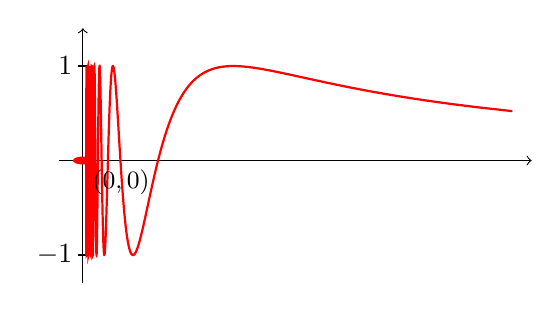
\begin{tikzpicture}[xscale=3, yscale=1.2]
\draw[->] (-0.1,0) -- (1.9,0);
\draw[->] (0,-1.3) -- (0,1.4);
\draw (-0.02,1) -- (0.02,1) node[left=2pt] {$1$};
\draw (-0.02,-1) -- (0.02,-1) node[left=2pt] {$-1$};
\draw[red, thick, samples=1500, domain=0.55:70, variable=\t] plot ({1/\t}, {sin(\t r)});
\fill[red] (0,0) circle (1.2pt);
\node[below right, font=\small] at (0,0) {$(0,0)$};
\end{tikzpicture}
